\addcontentsline{toc}{section}{Вариант 2}
\section*{Вариант 2}

\subsubsection*{1}

\textit{Задание.} Из множества $ \left\{ 1, 2, 3, 4, 5 \right\} $ независимо друг от друга выбирают число $ \xi $ и число $ \eta $.
Найдите вероятность того, что число $ \xi^2 - \eta^2$ делится на 2.

\textit{Решение.}
Пространством элементарных исходов является
$ \Omega = \\
= \left\{ \left( \xi, \eta \right): \, \xi, \eta \in \left\{ 1, 2, 3, 4, 5 \right\} \right\} $.
На каждом из двух мест может стоять любая из данных пяти цифр, поэтому $ \left| \Omega \right| = 5^2$.

Рассмотрим событие $A = \left\{ \left( \xi, \eta \right) \in \Omega: \, \left( \xi^2 - \eta^2 \right) \vdots 2 \right\} $.
Его наступлению способствуют такие пары чисел:
$ \left( 1, 1 \right), \left( 2, 2 \right),
\left( 3, 3 \right), \left( 4, 4 \right),
\left( 5, 5 \right), \left( 2, 4 \right),
\left( 4, 2 \right), \\
\left( 1, 3 \right), \left( 3, 1 \right), \left( 1, 5 \right), \left( 5, 1 \right), \left( 3, 5 \right), \left( 5, 3 \right) $.
Этих пар 13, поэтому $ \left| A \right| = 13$.

Тогда вероятность события равна
$$P \left( A \right) =
\frac{ \left| A \right| }{ \left| \Omega \right| } =
\frac{13}{5^2} =
\frac{13}{25}.$$

\subsubsection*{2}

\textit{Задание.} Подбросили два игральных кубика.
Найдите вероятность того, что на одном из них выпала тройка, если известно, что на кубиках выпало разное количество очков.

\textit{Решение.}
Пространство элементарных исходов имеет вид $ \Omega =  \\
= \left\{ \left( x_1, x_2 \right): x_1, x_2 \in \left\{ 1, 2, 3, 4, 5, 6\right\} \right\} $.
Оно содержит $ \left| \Omega \right| = 6^2$ элементов.

Введём событие $A = \left\{ \left( x_1, x_2 \right) \in \Omega: x_1 \neq x_2 \right\} =$ \{на кубиках выпало разное количество очков\}.
На одном из кубиков может выпасть любое число из шести --- 6 вариантов, а на втором кубике --- любое из оставшихся пяти --- 5 вариантов.
По правилу произведения $ \left| A \right| = 6 \cdot 5$.
Тогда вероятность этого события равна
$$P \left( A \right) =
\frac{ \left| A \right| }{ \left| \Omega \right| } =
\frac{6 \cdot 5}{6^2} =
\frac{5}{6}.$$

Введём событие $B = $ \{на одном из кубиков выпала тройка\}.
Опишем пересечение введённых событий: $A \cap B =  \\
= \left\{ \left( x_1, x_2 \right) \in \Omega: x_1 = 3 \neq x_2 or x_1 \neq 3 = x_2 \right\} $.
На одном из кубиков может быть только тройка --- 1 вариант.
А на другом кубике --- любая из оставшихся цифр --- 5 вариантов.
По правилу произведения $ \left| A \cap B \right| = 1 \cdot 5 \cdot C_2^1 = 5 \cdot 2$.
Тогда вероятность этого пересечения равна
$$P \left( A \cap B \right) =
\frac{ \left| A \cap B \right| }{ \left| \Omega \right| } =
\frac{5 \cdot 2}{6^2} =
\frac{5}{2 \cdot 6}.$$

Условная вероятность события $B$ при условии, что событие $A$ произошло, равна
$$P \left( \left. B \right| A \right) =
\frac{P \left( A \cap B \right) }{P \left( A \right) } =
\frac{ \frac{5}{6^2} }{ \frac{5}{6} } =
\frac{5 \cdot 6}{5 \cdot 6 \cdot 3} =
\frac{1}{3}.$$

\subsubsection*{3}

\textit{Задание.} Кандидат $A$ набрал на выборах 6 голосов, а кандидат $B$ --- 4 голоса (кандидатов было два и явка избирателей была 100\%).
Избиратели голосовали последовательно.
Найдите вероятность того, что кандидат $A$ всегда опережал $B$ не меньше, чем на один голос.

\textit{Решение.} Изобразим задачу на рисунке \ref{fig:23}.

\begin{figure}[h!]
  \centering
  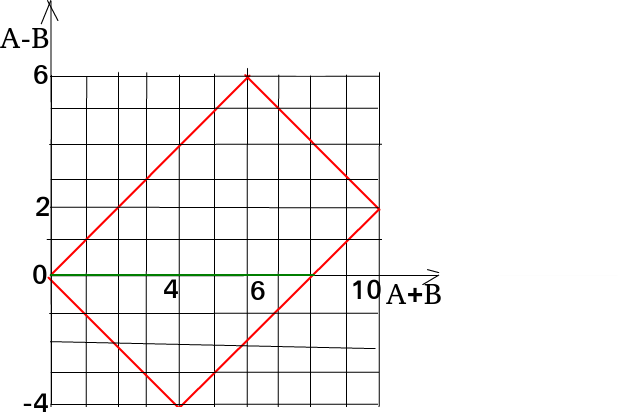
\includegraphics[width=.4\textwidth]{./pictures/t1v2_3.png}
  \caption{Пути}
  \label{fig:23}
\end{figure}

Красным обозначены граничные пути, зелёным --- линия, которой нельзя касаться.
В начале выборов разница у каждого кандидата было 0 голосов, в конце у кандидата $A$ было 6 голосов, а у кандидата $B$ --- 4 голоса.
Поэтому разность голосов в конце составляет 2 голоса.
Перевернём изображение (рис. \ref{fig:231}).

\begin{figure}[h!]
  \centering
  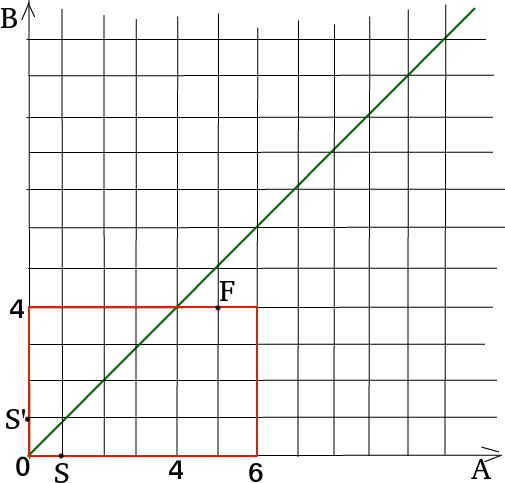
\includegraphics[width=.4\textwidth]{./pictures/t1v2_31.png}
  \caption{Метод отражений}
  \label{fig:231}
\end{figure}

Всего возможных путей есть столько, сколько путей из точки $S$ в точку $F$.
Их
$$ \left| \Omega \right| =
C_{6+4}^4 =
C_{10}^4 =
\frac{10!}{4! \cdot 6!} =
210.$$

Путей из точки $S$ в точку $F$ существует
$$ \left| S \rightarrow F \right| =
C_{5+4}^4 =
C_9^4 =
\frac{9!}{4! \cdot 5!} =
\frac{6 \cdot 7 \cdot 8 \cdot 9}{2 \cdot 3 \cdot 4} =
\frac{6 \cdot 7 \cdot 9}{2} =
2 \cdot 7 \cdot 9 =
149.$$
Путей, которые касаются диагонали ---
$$ \left| S' \rightarrow F \right| =
C_{5+3}^3 =
C_8^3 =
\frac{8!}{3! \cdot 5!} =
\frac{6 \cdot 7 \cdot 8}{2 \cdot 3} =
7 \cdot 8 =
56.$$

Тогда путей,
которые не пересекают диагональ и удовлетворяют указанному в условии событию $C$ будет
$ \left| C \right| =
\left| S \rightarrow F \right| - \left| S' \rightarrow F \right| =
189 - 56 =
133$.
И его вероятность равна
$$P \left( C \right) =
\frac{ \left| C \right| }{ \left| \Omega \right| } =
\frac{183}{210}.$$

\subsubsection*{4}

\textit{Задание.} На отрезок наугад брошено две точки.
Найдите вероятность того, что из трёх образованных отрезков можно составить треугольник.

\textit{Решение.} Пусть отрезок начинается в точке 0 и заканчивается в точке $c$.
Выбираем на нём наугад две точки: точку $a$ и точку $b$, причём $a$ лежит не правее $b$ (рис. \ref{fig:24}).

\begin{figure}[h!]
  \centering
  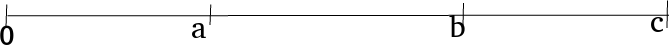
\includegraphics[width=.4\textwidth]{./pictures/t1v2_4.png}
  \caption{Отрезок $ \left[ 0, c \right] $}
  \label{fig:24}
\end{figure}

Тогда пространство элементарных исходов имеет вид $ \Omega =  \\
= \left\{ \left( a, b \right): 0 \leq a \leq b \leq c \right\} $.
Изобразив его на плоскости, видим, что это прямоугольный треугольник с катетами длиной $c$ (рис. \ref{fig:241}).

\begin{figure}[h!]
  \centering
  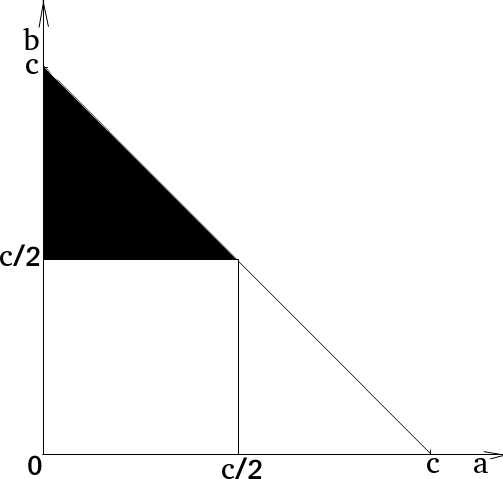
\includegraphics[width=.4\textwidth]{./pictures/t1v2_41.png}
  \caption{Пространство элементарных событий $ \Omega$ и событие $A$}
  \label{fig:241}
\end{figure}

Площадь треугольника равна
$$S_{ \Omega } =
\frac{1}{2} \cdot c \cdot c =
\frac{c^2}{2}.$$

Событие
$$A = \left\{ \left( a, b \right) \in \Omega: a \leq \frac{c}{2}, b \geq \frac{c}{2}, a \leq \frac{c}{2} + b \right\}.$$
Точки множества $A$ образуют прямоугольный треугольник с катетами $c/2$.
Его площадь равна
$$S_A =
\frac{1}{2} \cdot \frac{c}{2} \cdot \frac{c}{2} =
\frac{c^2}{8}.$$

Тогда вероятность события $A$ равна
$$P \left( A \right) =
\frac{S_A}{S_{ \Omega }} =
\frac{c^2}{8} \cdot \frac{2}{c^2} =
\frac{1}{4}.$$

\subsubsection*{5}

\textit{Задание.} В первой урне находятся 3 чёрных и 3 белых шарика, а во второй --- 2 чёрных и 3 белых шарика.
Из второй урны наугад вынули два шарика и переложили в первую.
После этого из первой урны вынимают два шарика.
Найдите вероятность того, что они окажутся разного цвета.

\textit{Решение.} Введём событие $A =$ \{вынутые после перекладывания шарики из первой урны окажутся разного цвета\}.
Введём гипотезы по поводу того,
каких цветов оказались шарики,
переложенные в первую урну из второй: $H_1 =$ \{чёрный, белый\}, $H_2 =$ \{белый, чёрный\}, $H_3 =$ \{чёрный, чёрный\}, $H_4 =$ \{белый, белый\}.
Найдём вероятности этих гипотез:
$$P \left( H_1 \right) =
\frac{2}{5} \cdot \frac{3}{4}, \,
P \left( H_2 \right) =
\frac{3}{5} \cdot \frac{2}{4}, \,
P \left( H_3 \right) =
\frac{2}{5}, \,
P \left( H_4 \right) =
\frac{3}{5}.$$

Найдём условные вероятности события $A$ при условии выполнения каждой из этих гипотез.
Пусть произошла гипотеза $H_1$.
Тогда в первой урне стало 4 чёрных и 4 белых шарика.
Вероятность того, что 2 вынутые шарика окажутся разного цвета, равна
$$P \left( \left. A \right| H_1 \right) =
\frac{4}{8} \cdot \frac{4}{7} \cdot 2.$$
Пусть произошла гипотеза $H_2$.
Тогда в первой урне стало 4 чёрных и 4 белых шарика.
Вероятность того, что 2 вынутые шарика окажутся разного цвета, равна
$$P \left( \left. A \right| H_2 \right) =
\frac{4}{8} \cdot \frac{4}{7} \cdot 2.$$
Пусть произошла гипотеза $H_3$.
Тогда в первой урне стало 5 чёрных и 3 белых шарика.
Вероятность того, что 2 вынутые шарика окажутся разного цвета, равна
$$P \left( \left. A \right| H_3 \right) =
\frac{5}{8} \cdot \frac{3}{7} \cdot 2.$$
Пусть произошла гипотеза $H_4$.
Тогда в первой урне стало 3 чёрных и 5 белых шарика.
Вероятность того, что 2 вынутые шарика окажутся разного цвета, равна
$$P \left( \left. A \right| H_4 \right) =
\frac{3}{8} \cdot \frac{5}{7} \cdot 2.$$

По формуле для полной вероятности
\begin{equation*}
\begin{split}
P \left( A \right) =
\sum \limits_{i=1}^4 P \left( H_i \right) \cdot P \left( \left. A \right| H_i \right).
\end{split}
\end{equation*}
